% answers.tex —— 2009 年·普通高等学校招生考试·安徽卷·文科 · 参考答案与详细解析片段
% 由 tools/generate_projects.py 依来源总账自 2009/2009_数学真题_安徽文_试题.md + 2009/2009_数学真题_安徽文_解析正文.md + 2009/2009_数学真题_安徽文_答案要点.md 生成，勿手改（改源 MD 后重跑）


\begin{gktip}
固定候选 PDF 仅含题面，无答案、解析和评分标准，原卷亦未标分值；以下为非官方编者独立推导，官方答案字段为空。题面文字层只作定位，分数、根号、下标与四幅图均以 600 dpi 原页复核。
\end{gktip}

\begin{answer}
\gksolhead{1}{}

\textbf{题目}：

$\mathrm i$ 是虚数单位，$\mathrm i(1+\mathrm i)$ 等于（　）

（A）$1+\mathrm i$

（B）$-1-\mathrm i$

（C）$1-\mathrm i$

（D）$-1+\mathrm i$

\Needspace{4\baselineskip}
\textbf{解析}

\nopagebreak[4]
\[\mathrm i(1+\mathrm i)=\mathrm i+\mathrm i^2=-1+\mathrm i,\]

选 D。

\gkanswer{答案：D。}

\end{answer}
\begin{answer}
\gksolhead{2}{}

\textbf{题目}：

若集合 $A=\left\{x\mid (2x+1)(x-3)<0\right\}$，$B=\{x\in\mathbf N_+\mid x\leqslant5\}$，则 $A\cap B$ 是（　）

（A）$\{1,2,3\}$

（B）$\{1,2\}$

（C）$\{4,5\}$

（D）$\{1,2,3,4,5\}$

\Needspace{4\baselineskip}
\textbf{解析}

\nopagebreak[4]
\[(2x+1)(x-3)<0\iff -\frac12<x<3,\]

\Needspace{5\baselineskip}
故

\nopagebreak[4]
\[A=\left(-\frac12,3\right).\]

\Needspace{5\baselineskip}
又 $B=\{x\in\mathbf N_+\mid x\leqslant5\}=\{1,2,3,4,5\}$，所以

\nopagebreak[4]
\[A\cap B=\{1,2\},\]

选 B。

\gkanswer{答案：B。}

\end{answer}
\begin{answer}
\gksolhead{3}{}

\textbf{题目}：

不等式组 $\begin{cases}x\geqslant0,\\ x+3y\geqslant4,\\ 3x+y\leqslant4\end{cases}$ 所表示的平面区域的面积等于（　）

（A）$\frac32$

（B）$\frac23$

（C）$\frac43$

（D）$\frac34$

\Needspace{4\baselineskip}
\textbf{解析}

先求三条边界两两的交点：

\begin{itemize}
\item $x=0$ 与 $x+3y=4$：$(0,\frac43)$；
\item $x=0$ 与 $3x+y=4$：$(0,4)$；
\item $x+3y=4$ 与 $3x+y=4$：相减得 $2x-2y=0$，即 $x=y$，代回得 $(1,1)$。
\end{itemize}

\Needspace{5\baselineskip}
可行域是以上三点为顶点的三角形。以 $x=0$ 上的边为底，底长 $4-\frac43=\frac83$，第三个顶点到该底的距离为 $1$，故

\nopagebreak[4]
\[S=\frac12\cdot\frac83\cdot1=\frac43,\]

选 C。

\gkanswer{答案：C。}

\end{answer}
\begin{answer}
\gksolhead{4}{}

\textbf{题目}：

「$a+c>b+d$」是「$a>b$ 且 $c>d$」的（　）

（A）必要不充分条件

（B）充分不必要条件

（C）充分必要条件

（D）既不充分也不必要条件

\Needspace{4\baselineskip}
\textbf{解析}

若 $a>b$ 且 $c>d$，两式相加得 $a+c>b+d$，故「$a+c>b+d$」是必要条件。

反之不成立。取 $a=1$、$b=2$、$c=5$、$d=0$，则 $a+c=6$、$b+d=2$，有 $a+c>b+d$，但 $a>b$ 不成立，更谈不上「$a>b$ 且 $c>d$」。故不充分。

综上为必要不充分条件，选 A。

\gkanswer{答案：A。}

\end{answer}
\begin{answer}
\gksolhead{5}{}

\textbf{题目}：

已知 $\{a_n\}$ 为等差数列，$a_1+a_3+a_5=105$，$a_2+a_4+a_6=99$，则 $a_{20}$ 等于（　）

（A）$-1$

（B）$1$

（C）$3$

（D）$7$

\Needspace{4\baselineskip}
\textbf{解析}

\Needspace{5\baselineskip}
等差数列中

\nopagebreak[4]
\[a_1+a_3+a_5=3a_3=105\ \Longrightarrow\ a_3=35,\]

\nopagebreak[4]
\[a_2+a_4+a_6=3a_4=99\ \Longrightarrow\ a_4=33 .\]

\Needspace{5\baselineskip}
故公差

\nopagebreak[4]
\[d=a_4-a_3=-2,\]

\nopagebreak[4]
\[a_{20}=a_3+17d=35-34=1,\]

选 B。

\gkanswer{答案：B。}

\end{answer}
\begin{answer}
\gksolhead{6}{}

\textbf{题目}：

下列曲线中离心率为 $\dfrac{\sqrt6}{2}$ 的是（　）

（A）$\frac{x^2}{2}-\frac{y^2}{4}=1$

（B）$\frac{x^2}{4}-\frac{y^2}{2}=1$

（C）$\frac{x^2}{4}-\frac{y^2}{6}=1$

（D）$\frac{x^2}{4}-\frac{y^2}{10}=1$

\Needspace{4\baselineskip}
\textbf{解析}

\Needspace{5\baselineskip}
对双曲线 $\frac{x^2}{a^2}-\frac{y^2}{b^2}=1$ 有 $c^2=a^2+b^2$，

\nopagebreak[4]
\[e^2=\frac{c^2}{a^2}=1+\frac{b^2}{a^2}.\]

由 $e=\frac{\sqrt6}{2}$ 得 $e^2=\frac32$，故 $b^2=\frac12a^2$。

逐项检验：

\begin{itemize}
\item (A) $\frac{x^2}{2}-\frac{y^2}{4}=1$：$a^2=2$、$b^2=4$，$e^2=1+2=3$；
\item (B) $\frac{x^2}{4}-\frac{y^2}{2}=1$：$a^2=4$、$b^2=2$，$e^2=1+\frac12=\frac32$；
\item (C) $\frac{x^2}{4}-\frac{y^2}{6}=1$：$e^2=1+\frac32=\frac52$；
\item (D) $\frac{x^2}{4}-\frac{y^2}{10}=1$：$e^2=1+\frac52=\frac72$。
\end{itemize}

只有 (B) 符合，选 B。

\gkanswer{答案：B。}

\end{answer}
\begin{answer}
\gksolhead{7}{}

\textbf{题目}：

直线 $l$ 过点 $(-1,2)$ 且与直线 $2x-3y+4=0$ 垂直，则 $l$ 的方程是（　）

（A）$3x+2y-1=0$

（B）$3x+2y+7=0$

（C）$2x-3y+5=0$

（D）$2x-3y+8=0$

\Needspace{4\baselineskip}
\textbf{解析}

\Needspace{5\baselineskip}
$2x-3y+4=0$ 的斜率为 $\frac23$，故与它垂直的直线斜率为 $-\frac32$。由点斜式

\nopagebreak[4]
\[y-2=-\frac32(x+1),\]

\Needspace{5\baselineskip}
即

\nopagebreak[4]
\[3x+2y-1=0,\]

选 A。

\gkanswer{答案：A。}

\end{answer}
\begin{answer}
\gksolhead{8}{}

\textbf{题目}：

设 $a<b$，函数 $y=(x-a)^2(x-b)$ 的图象可能是（　）
\nopagebreak[4]
\begin{center}% 2009 年安徽卷文科第 8 题：y=(x-a)^2(x-b)（a<b）的四个候选图象。
% 来源 PDF：普通高考/2009/2009安徽文.pdf，SHA256 83b982d22fd84a0158f909bce3d1f62e1fa228868e7915ded21e7a5ed9774897
% 原页：第 1 页（A3 三栏）第 1 栏下部与第 2 栏顶部，印刷页 497。
% 重绘依据：按原图四幅小图 2×2 排布，a 靠近原点、b 在右。(A) 与 x 轴有三个不同交点；
%   (B) 在 a 处穿过、在 b 处与 x 轴相切且开口向下；(C) 在 a 处与 x 轴相切（局部极大为 0）、
%   在 b 处自下而上穿过；(D) 在 a 处穿过、在 b 处相切（局部极小为 0）。
\begin{tikzpicture}[semithick, every node/.style={inner sep=1.1pt, font=\small}]
  % ---------- (A) ----------
  \begin{scope}[shift={(0,0)}, x=0.62cm, y=0.62cm]
    \begin{scope}
      \clip (-1.35,-2.35) rectangle (3.55,2.35);
      \draw[domain=-1.15:3.4,samples=200,smooth,variable=\x]
        plot (\x, {0.7*(-(\x+0.5))*(\x-0.35)*(\x-2.2)});
    \end{scope}
    \draw[-{Stealth}] (-1.3,0) -- (3.5,0) node[right] {$x$};
    \draw[-{Stealth}] (0,-2.25) -- (0,2.25) node[above] {$y$};
    \node[anchor=north east] at (-0.06,-0.08) {$O$};
    \node[below] at (0.75,-0.06) {$a$};
    \node[below] at (2.2,-0.06) {$b$};
    \node at (1.2,-3.05) {(A)};
  \end{scope}
  % ---------- (B) ----------
  \begin{scope}[shift={(5.0,0)}, x=0.62cm, y=0.62cm]
    \begin{scope}
      \clip (-1.35,-2.35) rectangle (3.55,2.35);
      \draw[domain=-1.15:3.4,samples=200,smooth,variable=\x]
        plot (\x, {0.7*(-(\x-0.35))*(\x-2.2)*(\x-2.2)});
    \end{scope}
    \draw[-{Stealth}] (-1.3,0) -- (3.5,0) node[right] {$x$};
    \draw[-{Stealth}] (0,-2.25) -- (0,2.25) node[above] {$y$};
    \node[anchor=north east] at (-0.06,-0.08) {$O$};
    \node[below] at (0.75,-0.06) {$a$};
    \node[below] at (2.2,-0.06) {$b$};
    \node at (1.2,-3.05) {(B)};
  \end{scope}
  % ---------- (C) ----------
  \begin{scope}[shift={(0,-4.2)}, x=0.62cm, y=0.62cm]
    \begin{scope}
      \clip (-1.35,-2.35) rectangle (3.55,2.35);
      \draw[domain=-1.15:3.4,samples=200,smooth,variable=\x]
        plot (\x, {0.7*(\x-0.35)*(\x-0.35)*(\x-2.2)});
    \end{scope}
    \draw[-{Stealth}] (-1.3,0) -- (3.5,0) node[right] {$x$};
    \draw[-{Stealth}] (0,-2.25) -- (0,2.25) node[above] {$y$};
    \node[anchor=north east] at (-0.06,-0.08) {$O$};
    \node[below] at (0.75,-0.06) {$a$};
    \node[below] at (2.2,-0.06) {$b$};
    \node at (1.2,-3.05) {(C)};
  \end{scope}
  % ---------- (D) ----------
  \begin{scope}[shift={(5.0,-4.2)}, x=0.62cm, y=0.62cm]
    \begin{scope}
      \clip (-1.35,-2.35) rectangle (3.55,2.35);
      \draw[domain=-1.15:3.4,samples=200,smooth,variable=\x]
        plot (\x, {0.7*(\x-0.35)*(\x-2.2)*(\x-2.2)});
    \end{scope}
    \draw[-{Stealth}] (-1.3,0) -- (3.5,0) node[right] {$x$};
    \draw[-{Stealth}] (0,-2.25) -- (0,2.25) node[above] {$y$};
    \node[anchor=north east] at (-0.06,-0.08) {$O$};
    \node[below] at (0.75,-0.06) {$a$};
    \node[below] at (2.2,-0.06) {$b$};
    \node at (1.2,-3.05) {(D)};
  \end{scope}
\end{tikzpicture}
\end{center}
\nopagebreak[4]
\Needspace{4\baselineskip}
\textbf{解析}

记 $f(x)=(x-a)^2(x-b)$，$a<b$。

因 $(x-a)^2\geqslant0$，故：

\begin{itemize}
\item $x<b$ 时 $f(x)\leqslant0$，等号仅在 $x=a$ 处成立，即在 $x=a$ 处图象与 $x$ 轴相切，且该点为局部极大值 $0$；
\item $x>b$ 时 $f(x)>0$，即在 $x=b$ 处图象自下而上穿过 $x$ 轴；
\item 在 $a<x<b$ 上 $f(x)<0$，极小值点为 $x=\frac{a+2b}{3}$；
\item $x\to-\infty$ 时 $f\to-\infty$，$x\to+\infty$ 时 $f\to+\infty$。
\end{itemize}

对照四个候选：

\begin{itemize}
\item (A) 与 $x$ 轴有三个不同的交点，说明三个单根，不合；
\item (B) 在 $a$ 处穿过、在 $b$ 处相切，且 $x\to-\infty$ 时 $f\to+\infty$，形如 $-(x-a)(x-b)^2$，不合；
\item (C) 在 $a$ 处相切（局部极大为 $0$）、在 $b$ 处自下而上穿过，且两端走向与 $f$ 一致，符合；
\item (D) 在 $a$ 处穿过、在 $b$ 处相切（局部极小为 $0$），形如 $(x-a)(x-b)^2$，不合。
\end{itemize}

故选 C。

\gkanswer{答案：C。}

\end{answer}
\begin{answer}
\gksolhead{9}{}

\textbf{题目}：

设函数 $f(x)=\dfrac{\sin\theta}{3}x^3+\dfrac{\sqrt3\cos\theta}{2}x^2+\tan\theta$，其中 $\theta\in\left[0,\dfrac{5\pi}{12}\right]$，则导数 $f'(1)$ 的取值范围是（　）

（A）$[-2,2]$

（B）$[\sqrt2,\sqrt3]$

（C）$[\sqrt3,2]$

（D）$[\sqrt2,2]$

\Needspace{4\baselineskip}
\textbf{解析}

\nopagebreak[4]
\[f'(x)=\sin\theta\cdot x^2+\sqrt3\cos\theta\cdot x,\]

\nopagebreak[4]
\[f'(1)=\sin\theta+\sqrt3\cos\theta=2\sin\left(\theta+\frac\pi3\right).\]

\Needspace{5\baselineskip}
当 $\theta\in\left[0,\frac{5\pi}{12}\right]$ 时，

\nopagebreak[4]
\[\theta+\frac\pi3\in\left[\frac\pi3,\frac{3\pi}{4}\right].\]

\Needspace{5\baselineskip}
在此区间上 $\sin$ 先由 $\frac{\sqrt3}{2}$ 增到 $1$（在 $\frac\pi2$ 处），再减到 $\frac{\sqrt2}{2}$，故

\nopagebreak[4]
\[2\sin\left(\theta+\frac\pi3\right)\in[\sqrt2,2],\]

选 D。

\gkanswer{答案：D。}

\end{answer}
\begin{answer}
\gksolhead{10}{}

\textbf{题目}：

考察正方体 $6$ 个面的中心，从中任意选 $3$ 个点连成三角形，再把剩下的 $3$ 个点也连成三角形，则所得的两个三角形全等的概率等于（　）

（A）$1$

（B）$\frac12$

（C）$\frac13$

（D）$0$

\Needspace{4\baselineskip}
\textbf{解析}

\Needspace{5\baselineskip}
以正方体中心为原点建系，六个面的中心为

\nopagebreak[4]
\[\pm\boldsymbol e_1,\ \pm\boldsymbol e_2,\ \pm\boldsymbol e_3,\]

即正八面体的六个顶点。任取三点必不共线，都构成三角形。

\begin{itemize}
\item 若三点含一对对径点，例如 $\boldsymbol e_1,-\boldsymbol e_1,\boldsymbol e_2$，则三边长为 $2,\sqrt2,\sqrt2$；其补集 $\{-\boldsymbol e_2,\boldsymbol e_3,-\boldsymbol e_3\}$ 也含一对对径点，三边长同样为 $2,\sqrt2,\sqrt2$，两者全等。
\item 若三点不含对径点，则每条轴各取一个顶点，两两距离都是 $\sqrt2$，为等边三角形；其补集同样每条轴各取一个，也是等边三角形，两者全等。
\end{itemize}

故无论怎样选取，所得两个三角形都全等，概率为 $1$，选 A。

\gkanswer{答案：A。}

\end{answer}
\begin{answer}
\gksolhead{11}{}

\textbf{题目}：

在空间直角坐标系中，已知点 $A(1,0,2)$，$B(1,-3,1)$，点 $M$ 在 $y$ 轴上，且 $M$ 到 $A$ 与到 $B$ 的距离相等，则 $M$ 的坐标是\gkblank{}．

\Needspace{4\baselineskip}
\textbf{解析}

\Needspace{5\baselineskip}
设 $M(0,y,0)$。由 $|MA|=|MB|$：

\nopagebreak[4]
\[(1-0)^2+(0-y)^2+(2-0)^2=(1-0)^2+(-3-y)^2+(1-0)^2,\]

\nopagebreak[4]
\[1+y^2+4=1+(y+3)^2+1 .\]

\Needspace{5\baselineskip}
化简

\nopagebreak[4]
\[y^2+5=y^2+6y+11\ \Longrightarrow\ 6y=-6\ \Longrightarrow\ y=-1 .\]

故 $M(0,-1,0)$。

\gkanswer{答案：$(0,-1,0)$。}

\end{answer}
\begin{answer}
\gksolhead{12}{}

\textbf{题目}：

程序框图（即算法流程图）如图所示，其输出结果是\gkblank{}．
\nopagebreak[4]
\begin{center}% 2009 年安徽卷文科第 12 题：程序框图，输出 a 的值。
% 来源 PDF：普通高考/2009/2009安徽文.pdf，SHA256 83b982d22fd84a0158f909bce3d1f62e1fa228868e7915ded21e7a5ed9774897
% 原页：第 1 页（A3 三栏）第 2 栏中部，印刷页 497。
% 重绘依据：开始 → a=1 → a=2a+1 → 判断 a>100；否（左）回到 a=2a+1，是（下）→ 输出 a → 结束。
\begin{tikzpicture}[scale=0.9, semithick, >=Stealth,
  node distance=5mm, every node/.style={inner sep=3pt, font=\small}]
  \node (start) [draw, rounded corners=4pt, minimum width=1.9cm, minimum height=0.62cm] {开始};
  \node (init) [draw, minimum width=1.9cm, minimum height=0.62cm, below=of start] {$a=1$};
  \node (step) [draw, minimum width=2.6cm, minimum height=0.62cm, below=of init] {$a=2a+1$};
  \node (cond) [draw, diamond, aspect=2.0, minimum width=2.6cm, minimum height=0.95cm, below=of step] {$a>100$};
  \node (out) [draw, trapezium, trapezium left angle=70, trapezium right angle=110,
    minimum width=2.4cm, minimum height=0.62cm, below=of cond] {输出 $a$};
  \node (end) [draw, rounded corners=4pt, minimum width=1.9cm, minimum height=0.62cm, below=of out] {结束};
  \draw[->] (start) -- (init);
  \draw[->] (init) -- (step);
  \draw[->] (step) -- (cond);
  \draw[->] (cond) -- (out);
  \node[anchor=west] at ($(cond.south)!0.5!(out.north)+(16pt,-4pt)$) {是};
  \draw[->] (cond.west) -- ++(-0.85,0) |- node[pos=0.25, left] {否} (step.west);
  \draw[->] (out) -- (end);
\end{tikzpicture}
\end{center}
\nopagebreak[4]
\Needspace{4\baselineskip}
\textbf{解析}

\Needspace{5\baselineskip}
初始 $a=1$，每次执行 $a\leftarrow2a+1$：

\nopagebreak[4]
\[1\to3\to7\to15\to31\to63\to127 .\]

判断条件为 $a>100$：前几次都不满足，继续循环；当 $a=127$ 时满足，跳出并输出 $127$。

\gkanswer{答案：$127$。}

\end{answer}
\begin{answer}
\gksolhead{13}{}

\textbf{题目}：

从长度分别为 $2,3,4,5$ 的四条线段中任意取出三条，则以这三条线段为边可以构成三角形的概率是\gkblank{}．

\Needspace{4\baselineskip}
\textbf{解析}

四条线段中任取三条，共 $\mathrm C_4^3=4$ 种组合。逐组检验两边之和大于第三边：

\begin{itemize}
\item $2,3,4$：$2+3>4$，可以；
\item $2,3,5$：$2+3=5$，不可以；
\item $2,4,5$：$2+4>5$，可以；
\item $3,4,5$：$3+4>5$，可以。
\end{itemize}

故所求概率为 $\frac34$。

\gkanswer{答案：$\frac34$。}

\end{answer}
\begin{answer}
\gksolhead{14}{}

\textbf{题目}：

在平行四边形 $ABCD$ 中，$E$ 和 $F$ 分别是边 $CD$ 和 $BC$ 的中点．若 $\overrightarrow{AC}=\lambda\overrightarrow{AE}+\mu\overrightarrow{AF}$，其中 $\lambda,\mu\in\mathbf R$，则 $\lambda+\mu=$\gkblank{}．

\Needspace{4\baselineskip}
\textbf{解析}

\Needspace{5\baselineskip}
记 $\overrightarrow{AB}=\boldsymbol b$、$\overrightarrow{AD}=\boldsymbol d$，则

\nopagebreak[4]
\[\overrightarrow{AC}=\boldsymbol b+\boldsymbol d .\]

\Needspace{5\baselineskip}
由中点公式

\nopagebreak[4]
\[\overrightarrow{AE}=\overrightarrow{AD}+\frac12\overrightarrow{DC}=\boldsymbol d+\frac12\boldsymbol b,\]

\nopagebreak[4]
\[\overrightarrow{AF}=\overrightarrow{AB}+\frac12\overrightarrow{BC}=\boldsymbol b+\frac12\boldsymbol d .\]

\Needspace{5\baselineskip}
设 $\overrightarrow{AC}=\lambda\overrightarrow{AE}+\mu\overrightarrow{AF}$，即

\nopagebreak[4]
\[\boldsymbol b+\boldsymbol d=\left(\frac\lambda2+\mu\right)\boldsymbol b+\left(\lambda+\frac\mu2\right)\boldsymbol d .\]

\Needspace{5\baselineskip}
因 $\boldsymbol b,\boldsymbol d$ 不共线，比较系数得

\nopagebreak[4]
\[\frac\lambda2+\mu=1,\qquad \lambda+\frac\mu2=1 .\]

\Needspace{5\baselineskip}
两式相减得 $\frac{\mu-\lambda}{2}=0$，故 $\lambda=\mu$，代回得 $\frac32\lambda=1$，即 $\lambda=\mu=\frac23$，所以

\nopagebreak[4]
\[\lambda+\mu=\frac43 .\]

\gkanswer{答案：$\frac43$。}

\end{answer}
\begin{answer}
\gksolhead{15}{}

\textbf{题目}：

对于四面体 $ABCD$，下列命题正确的是\gkblank{}．（写出所有正确命题的编号）

① 相对棱 $AB$ 与 $CD$ 所在的直线异面；

② 由顶点 $A$ 作四面体的高，其垂足是 $\triangle BCD$ 的三条高线的交点；

③ 若分别作 $\triangle ABC$ 和 $\triangle ABD$ 的边 $AB$ 上的高，则这两条高所在直线异面；

④ 任何三个面的面积之和都大于第四个面的面积；

⑤ 分别作三组相对棱中点的连线，所得的三条线段相交于一点．

\Needspace{4\baselineskip}
\textbf{解析}

① 正确：四面体中没有两条相对棱共面，相对棱所在直线必异面。

② 错误：设 $A$ 在平面 $BCD$ 上的垂足为 $H$，则 $AH\perp$ 平面 $BCD$。由三垂线定理，$H$ 为 $\triangle BCD$ 的垂心当且仅当 $AB\perp CD$、$AC\perp BD$、$AD\perp BC$ 同时成立（垂心四面体），一般四面体不满足。

③ 错误：两条高都垂直于 $AB$，分别位于平面 $ABC$ 与 $ABD$ 内；若两高的垂足重合，则两直线交于该点，不是异面直线。

④ 正确：设最大面为 $BCD$，由 $A$ 向平面 $BCD$ 作垂线，其余三个面在平面 $BCD$ 上的投影覆盖 $\triangle BCD$（可能重叠），故 $S_{\triangle BCD}\leqslant S_{\triangle ABC}+S_{\triangle ACD}+S_{\triangle ABD}$，即任何三个面的面积之和不小于第四个面（严格情形下大于）。

⑤ 正确：设 $E,F,G,H,I,J$ 分别为 $AB,CD,AC,BD,AD,BC$ 的中点，则 $EF$、$GH$、$IJ$ 三线都经过四面体重心且被重心平分，故交于一点。

故填 ①④⑤。

\gkanswer{答案：①④⑤。}

\end{answer}
\begin{answer}
\gksolhead{16}{}

\textbf{题目}：

在 $\triangle ABC$ 中，$C-A=\dfrac{\pi}{2}$，$\sin B=\dfrac13$．

（1）求 $\sin A$ 的值；

（2）设 $AC=\sqrt6$，求 $\triangle ABC$ 的面积．

\Needspace{4\baselineskip}
\textbf{解析}

\Needspace{5\baselineskip}
（1）由 $C=A+\frac\pi2$ 及 $A+B+C=\pi$：

\nopagebreak[4]
\[A+B+A+\frac\pi2=\pi\ \Longrightarrow\ B=\frac\pi2-2A .\]

\Needspace{5\baselineskip}
于是

\nopagebreak[4]
\[\sin B=\sin\left(\frac\pi2-2A\right)=\cos2A=1-2\sin^2A=\frac13,\]

\Needspace{5\baselineskip}
故

\nopagebreak[4]
\[\sin^2A=\frac13 .\]

\Needspace{5\baselineskip}
由 $B>0$ 得 $2A<\frac\pi2$，即 $A$ 为锐角，所以

\nopagebreak[4]
\[\sin A=\frac{\sqrt3}{3},\qquad \cos A=\sqrt{1-\frac13}=\frac{\sqrt6}{3}.\]

\Needspace{5\baselineskip}
（2）

\nopagebreak[4]
\[\sin C=\sin\left(A+\frac\pi2\right)=\cos A=\frac{\sqrt6}{3}.\]

\Needspace{5\baselineskip}
由正弦定理

\nopagebreak[4]
\[\frac{a}{\sin A}=\frac{b}{\sin B},\]

\Needspace{5\baselineskip}
其中 $b=AC=\sqrt6$、$\sin B=\frac13$，故

\nopagebreak[4]
\[\frac{a}{\sqrt3/3}=\frac{\sqrt6}{1/3}\ \Longrightarrow\ a=3\sqrt2 .\]

\Needspace{5\baselineskip}
于是

\nopagebreak[4]
\[S=\frac12ab\sin C=\frac12\cdot3\sqrt2\cdot\sqrt6\cdot\frac{\sqrt6}{3}=3\sqrt2 .\]

\gkanswer{答案：（1）$\dfrac{\sqrt3}{3}$；（2）$3\sqrt2$。}

\end{answer}
\begin{answer}
\gksolhead{17}{}

\textbf{题目}：

某良种培育基地正在培育一种小麦新品种 $A$，将其与原有的一个优良品种 $B$ 进行对照试验，两种小麦各种植了 $25$ 亩，所得亩产数据（单位：千克）如下：

品种 $A$：$357$，$359$，$367$，$368$，$375$，$388$，$392$，$399$，$400$，$405$，$412$，$414$，$415$，$421$，$423$，$423$，$427$，$430$，$430$，$434$，$443$，$445$，$451$，$454$．

品种 $B$：$363$，$371$，$374$，$383$，$385$，$386$，$391$，$392$，$394$，$395$，$397$，$397$，$400$，$401$，$401$，$403$，$406$，$407$，$410$，$412$，$415$，$416$，$422$，$430$．

（1）完成所附的茎叶图；

（2）用茎叶图处理现有的数据，有什么优点？

（3）通过观察茎叶图，对品种 $A$ 与 $B$ 的亩产量及其稳定性进行比较，写出统计结论．
\nopagebreak[4]
\begin{center}% 2009 年安徽卷文科第 17 题：待填写的茎叶图空白表。
% 来源 PDF：普通高考/2009/2009安徽文.pdf，SHA256 83b982d22fd84a0158f909bce3d1f62e1fa228868e7915ded21e7a5ed9774897
% 原页：第 1 页（A3 三栏）第 3 栏下部，印刷页 497。
% 重绘依据：表头左「A」右「B」，中间为茎（35–45），两侧留空供填写叶；按原图保留竖线与横线。
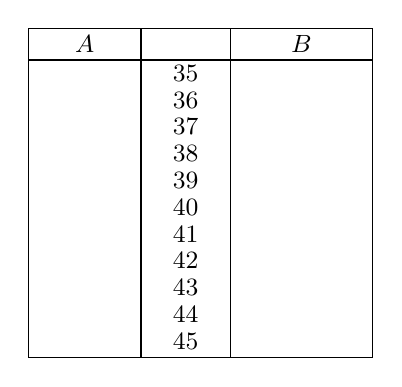
\begin{tikzpicture}[scale=0.95, semithick, every node/.style={inner sep=2.2pt, font=\small}]
  \draw (0,0) rectangle (4.6,-4.4);
  \draw (1.5,0) -- (1.5,-4.4);
  \draw (2.7,0) -- (2.7,-4.4);
  \draw (0,-0.42) -- (4.6,-0.42);
  \node at (0.75,-0.21) {$A$};
  \node at (3.65,-0.21) {$B$};
  \foreach \i/\s in {0/35,1/36,2/37,3/38,4/39,5/40,6/41,7/42,8/43,9/44,10/45} {
    \node at (2.1,{-0.42-(\i+0.5)*0.358}) {$\s$};
  }
\end{tikzpicture}
\end{center}
\nopagebreak[4]
\Needspace{4\baselineskip}
\textbf{解析}

（1）茎为百位与十位，叶为个位，按数据升序填写（原页 A、B 各印出 $24$ 个数据）：
\nopagebreak[4]
\begin{center}% 2009 年安徽卷文科第 17 题：按原卷印出的 24 个亩产数据填写的茎叶图（解答用）。
% 来源 PDF：普通高考/2009/2009安徽文.pdf，SHA256 83b982d22fd84a0158f909bce3d1f62e1fa228868e7915ded21e7a5ed9774897
% 原页：第 1 页（A3 三栏）第 3 栏下部，印刷页 497；题目数据见第 3 栏上部。
% 重绘依据：茎为十位与百位（35–45），叶为个位；A、B 两列按数据升序排列，逐项照录。
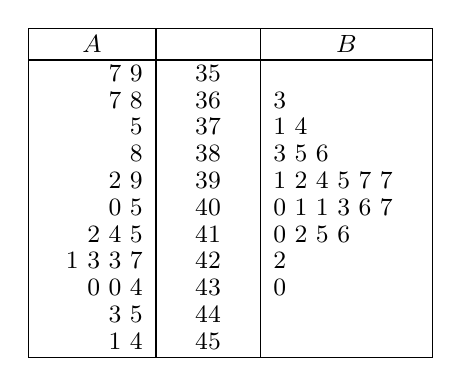
\begin{tikzpicture}[scale=0.95, semithick, every node/.style={inner sep=2.2pt, font=\small}]
  \draw (0,0) rectangle (5.4,-4.4);
  \draw (1.7,0) -- (1.7,-4.4);
  \draw (3.1,0) -- (3.1,-4.4);
  \draw (0,-0.42) -- (5.4,-0.42);
  \node at (0.85,-0.21) {$A$};
  \node at (4.25,-0.21) {$B$};
  \foreach \i/\s/\l/\r in {%
    0/35/{7\ 9}/{},%
    1/36/{7\ 8}/{3},%
    2/37/{5}/{1\ 4},%
    3/38/{8}/{3\ 5\ 6},%
    4/39/{2\ 9}/{1\ 2\ 4\ 5\ 7\ 7},%
    5/40/{0\ 5}/{0\ 1\ 1\ 3\ 6\ 7},%
    6/41/{2\ 4\ 5}/{0\ 2\ 5\ 6},%
    7/42/{1\ 3\ 3\ 7}/{2},%
    8/43/{0\ 0\ 4}/{0},%
    9/44/{3\ 5}/{},%
    10/45/{1\ 4}/{}} {
    \node[anchor=center] at (2.4,{-0.42-(\i+0.5)*0.358}) {$\s$};
    \node[anchor=east] at (1.62,{-0.42-(\i+0.5)*0.358}) {$\l$};
    \node[anchor=west] at (3.18,{-0.42-(\i+0.5)*0.358}) {$\r$};
  }
\end{tikzpicture}
\end{center}
\nopagebreak[4]
（2）茎叶图的优点是：既能反映数据的分布情况（集中与离散），又能保留每一个原始数据，便于记录与读取，且可随时补充新数据；用于两组数据对比时，可直接看出平均水平与稳定性的差异。

\Needspace{5\baselineskip}
（3）由茎叶图读得两组数据的和：

\nopagebreak[4]
\[\sum A=9832,\qquad \sum B=9551,\]

\Needspace{5\baselineskip}
故

\nopagebreak[4]
\[\bar x_A=\frac{9832}{24}\approx409.7,\qquad \bar x_B=\frac{9551}{24}\approx398.0 .\]

$A$ 的平均亩产高于 $B$。

再看离散程度：$A$ 的数据分布在 $357\sim454$，极差 $97$；$B$ 的数据分布在 $363\sim430$，极差 $67$，且 $B$ 的叶更集中于 $39$、$40$、$41$ 三行。故 $B$ 的亩产更稳定。

\gkanswer{答案：（1）茎叶图见解析版；（2）优点见下；（3）$A$ 的平均亩产高于 $B$，$B$ 的亩产更稳定。}

\end{answer}
\begin{answer}
\gksolhead{18}{}

\textbf{题目}：

已知椭圆 $\dfrac{x^2}{a^2}+\dfrac{y^2}{b^2}=1$（$a>b>0$）的离心率为 $\dfrac{\sqrt3}{3}$，以原点为圆心、椭圆短半轴长为半径的圆与直线 $y=x+2$ 相切．

（1）求 $a$ 与 $b$；

（2）设该椭圆的左、右焦点分别为 $F_1$ 和 $F_2$，直线 $l_1$ 过 $F_2$ 且与 $x$ 轴垂直，动直线 $l_2$ 与 $y$ 轴垂直，交 $l_1$ 于点 $P$．求线段 $PF_1$ 的垂直平分线与 $l_2$ 的交点 $M$ 的轨迹方程，并指明曲线类型．

\Needspace{4\baselineskip}
\textbf{解析}

\Needspace{5\baselineskip}
（1）圆 $x^2+y^2=b^2$ 与直线 $y=x+2$ 相切，圆心到直线的距离等于半径：

\nopagebreak[4]
\[b=\frac{|0-0+2|}{\sqrt{1^2+(-1)^2}}=\sqrt2 .\]

\Needspace{5\baselineskip}
又

\nopagebreak[4]
\[e^2=\frac{c^2}{a^2}=1-\frac{b^2}{a^2},\]

\Needspace{5\baselineskip}
由 $e=\frac{\sqrt3}{3}$ 得

\nopagebreak[4]
\[1-\frac{2}{a^2}=\frac13\ \Longrightarrow\ a^2=3,\]

故 $a=\sqrt3$、$b=\sqrt2$。

（2）$c=\sqrt{a^2-b^2}=1$，故 $F_1(-1,0)$、$F_2(1,0)$，且 $l_1:x=1$。

设 $l_2:y=t$（$t\neq0$），它与 $l_1$ 交于 $P(1,t)$。

\Needspace{5\baselineskip}
$PF_1$ 的中点 $N\left(0,\frac t2\right)$，$PF_1$ 的斜率为

\nopagebreak[4]
\[k_{PF_1}=\frac{t-0}{1-(-1)}=\frac t2,\]

\Needspace{5\baselineskip}
故 $PF_1$ 的垂直平分线斜率为 $-\frac2t$，方程为

\nopagebreak[4]
\[y-\frac t2=-\frac2t x .\]

\Needspace{5\baselineskip}
与 $y=t$ 联立：

\nopagebreak[4]
\[\frac t2=-\frac{2x}{t}\ \Longrightarrow\ x=-\frac{t^2}{4} .\]

\Needspace{5\baselineskip}
故 $M\left(-\frac{t^2}{4},t\right)$，消去 $t$ 得

\nopagebreak[4]
\[y^2=-4x .\]

轨迹是以原点为顶点、焦点为 $(-1,0)$、开口向左的抛物线。

\gkanswer{答案：（1）$a=\sqrt3$，$b=\sqrt2$；（2）$y^2=-4x$，是抛物线。}

\end{answer}
\begin{answer}
\gksolhead{19}{}

\textbf{题目}：

已知数列 $\{a_n\}$ 的前 $n$ 项和 $S_n=2n^2+2n$，数列 $\{b_n\}$ 的前 $n$ 项和 $T_n=2-b_n$．

（1）求数列 $\{a_n\}$ 与 $\{b_n\}$ 的通项公式；

（2）设 $c_n=a_{2n}^2\cdot b_n$，证明：当且仅当 $n\geqslant3$ 时，$c_{n+1}<c_n$．

\Needspace{4\baselineskip}
\textbf{解析}

\Needspace{5\baselineskip}
（1）$n\geqslant2$ 时，

\nopagebreak[4]
\[a_n=S_n-S_{n-1}=2n^2+2n-\left[2(n-1)^2+2(n-1)\right].\]

\Needspace{5\baselineskip}
展开

\nopagebreak[4]
\[2(n-1)^2+2(n-1)=2n^2-4n+2+2n-2=2n^2-2n,\]

\Needspace{5\baselineskip}
故

\nopagebreak[4]
\[a_n=(2n^2+2n)-(2n^2-2n)=4n .\]

$n=1$ 时 $a_1=S_1=4$，与上式一致，故 $a_n=4n$。

\Needspace{5\baselineskip}
对 $\{b_n\}$：$n=1$ 时 $b_1=T_1=2-b_1$，故 $b_1=1$。$n\geqslant2$ 时

\nopagebreak[4]
\[b_n=T_n-T_{n-1}=(2-b_n)-(2-b_{n-1})=b_{n-1}-b_n,\]

\Needspace{5\baselineskip}
故

\nopagebreak[4]
\[b_n=\frac12 b_{n-1},\]

\Needspace{5\baselineskip}
即 $\{b_n\}$ 是首项 $1$、公比 $\frac12$ 的等比数列，

\nopagebreak[4]
\[b_n=\left(\frac12\right)^{n-1}=2^{1-n}.\]

\Needspace{5\baselineskip}
（2）由（1）

\nopagebreak[4]
\[c_n=a_{2n}^2b_n=(8n)^2\cdot2^{1-n}=64n^2\cdot2^{1-n}.\]

\Needspace{5\baselineskip}
于是

\nopagebreak[4]
\[\frac{c_{n+1}}{c_n}=\frac{64(n+1)^2 2^{-n}}{64n^2 2^{1-n}}=\frac{(n+1)^2}{2n^2}.\]

\Needspace{5\baselineskip}
故

\nopagebreak[4]
\[c_{n+1}<c_n\iff (n+1)^2<2n^2\iff n^2-2n-1>0 .\]

\Needspace{5\baselineskip}
二次方程 $n^2-2n-1=0$ 的正根为 $1+\sqrt2\approx2.41$，故不等式对整数 $n$ 成立当且仅当

\nopagebreak[4]
\[n\geqslant3 .\]

即当且仅当 $n\geqslant3$ 时 $c_{n+1}<c_n$。

\gkanswer{答案：（1）$a_n=4n$，$b_n=2^{1-n}$；（2）证明见解析。}

\end{answer}
\begin{answer}
\gksolhead{20}{}

\textbf{题目}：

如图，$ABCD$ 是边长为 $2$ 的正方形，直线 $l$ 与平面 $ABCD$ 平行，$E$ 和 $F$ 是 $l$ 上的两个不同点，且 $EA=ED$，$FB=FC$．$E'$ 和 $F'$ 是平面 $ABCD$ 内的两点，$EE'$ 和 $FF'$ 都与平面 $ABCD$ 垂直．
\nopagebreak[4]
\begin{center}% 2009 年安徽卷文科第 20 题：正方形 ABCD 与平行直线 l 构成的六面体 ABCDEF。
% 来源 PDF：普通高考/2009/2009安徽文.pdf，SHA256 83b982d22fd84a0158f909bce3d1f62e1fa228868e7915ded21e7a5ed9774897
% 原页：第 2 页（A3 三栏）第 2 栏中部，印刷页 498。
% 重绘依据：正方形按斜投影画成平行四边形，A 左下、B 右下、C 右上、D 左上；l 为 AB 上方的水平直线，
%   E、F 在 l 上（F 在右、超出正方形右边界）；E′、F′ 在正方形平面内的中线上，
%   EE′、FF′ 画虚线，DC 画虚线（被遮挡）；实线为 AB、BC、AD 与 E、F 到 A、D、B、C 的连线。
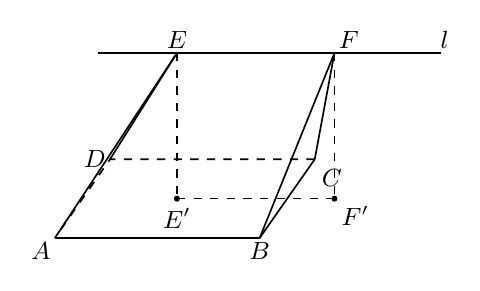
\begin{tikzpicture}[scale=1.0, semithick, every node/.style={inner sep=1.3pt, font=\small}]
  \coordinate (A) at (0,0);
  \coordinate (B) at (2.6,0);
  \coordinate (C) at (3.3,1.0);
  \coordinate (D) at (0.7,1.0);
  \coordinate (E) at (1.55,2.35);
  \coordinate (F) at (3.55,2.35);
  \coordinate (Ep) at (1.55,0.5);
  \coordinate (Fp) at (3.55,0.5);
  % 直线 l
  \draw (0.55,2.35) -- (4.9,2.35);
  \node[above] at (4.95,2.35) {$l$};
  % 正方形
  \draw (A) -- (B) -- (C);
  \draw[dashed] (C) -- (D) -- (A);
  % 棱
  \draw (A) -- (E);
  \draw (D) -- (E);
  \draw (B) -- (F);
  \draw (C) -- (F);
  \draw (E) -- (F);
  % 垂线
  \draw[dashed] (E) -- (Ep);
  \draw[dashed] (F) -- (Fp);
  % 中线
  \draw[dashed] (Ep) -- (Fp);
  \fill (Ep) circle (1.1pt);
  \fill (Fp) circle (1.1pt);
  \node[below left] at (A) {$A$};
  \node[below] at (B) {$B$};
  \node[anchor=north west] at ([xshift=1pt,yshift=-2pt]C) {$C$};
  \node[left] at (D) {$D$};
  \node[above] at (E) {$E$};
  \node[anchor=south west] at (F) {$F$};
  \node[below] at ([yshift=-2pt]Ep) {$E'$};
  \node[anchor=north west] at ([xshift=1pt,yshift=-1pt]Fp) {$F'$};
\end{tikzpicture}
\end{center}
\nopagebreak[4]
（1）证明：直线 $E'F'$ 垂直且平分线段 $AD$；

（2）若 $\angle EAD=\angle EAB=60^\circ$，$EF=2$，求多面体 $ABCDEF$ 的体积．

\Needspace{4\baselineskip}
\textbf{解析}

\Needspace{5\baselineskip}
（1）因 $EE'\perp$ 平面 $ABCD$，故 $\triangle EE'A$ 与 $\triangle EE'D$ 都是直角三角形：

\nopagebreak[4]
\[EA^2=EE'^2+E'A^2,\qquad ED^2=EE'^2+E'D^2 .\]

由 $EA=ED$ 得 $E'A=E'D$，故 $E'$ 在 $AD$ 的垂直平分线上。同理，由 $FB=FC$ 得 $F'$ 在 $BC$ 的垂直平分线上。

正方形 $ABCD$ 中 $AD\parallel BC$，且 $AD$ 与 $BC$ 的中点在平行于 $AB$ 的同一条直线上，故 $AD$ 与 $BC$ 的垂直平分线重合。于是 $E'$、$F'$ 都在这条重合的垂直平分线上，直线 $E'F'$ 即为它。该直线垂直于 $AD$ 且过 $AD$ 的中点，即垂直且平分线段 $AD$。

\Needspace{5\baselineskip}
（2）取 $A(0,0,0)$、$B(2,0,0)$、$C(2,2,0)$、$D(0,2,0)$。由（1），$E'$、$F'$ 都在直线 $y=1$ 上，设

\nopagebreak[4]
\[E'(s,1,0),\quad E(s,1,h),\quad F'(t,1,0),\quad F(t,1,h)\quad(h>0).\]

\Needspace{5\baselineskip}
\textbf{求 $s$ 与 $h$}：$\overrightarrow{AE}=(s,1,h)$、$\overrightarrow{AD}=(0,2,0)$、$\overrightarrow{AB}=(2,0,0)$。

\nopagebreak[4]
\[\cos\angle EAD=\frac{2}{2|AE|}=\frac12\ \Longrightarrow\ |AE|=2,\]

\nopagebreak[4]
\[\cos\angle EAB=\frac{2s}{2|AE|}=\frac12\ \Longrightarrow\ s=1 .\]

再由 $|AE|^2=1+1+h^2=4$ 得 $h=\sqrt2$。

\textbf{求体积}：$EF=|t-s|=2$，按图形取 $t=3$（取 $t=-1$ 时所得多面体是它关于平面 $x=1$ 的对称体，体积相同）。

\Needspace{5\baselineskip}
注意到

\nopagebreak[4]
\[\overrightarrow{AB}=\overrightarrow{DC}=\overrightarrow{EF}=(2,0,0),\]

三条侧棱平行且相等，故 $ABCDEF$ 是以 $\triangle ADE$ 为底面、侧棱长 $2$ 的直三棱柱，另一底面为 $\triangle BCF$。

\Needspace{5\baselineskip}
$AD=2$、$AE=2$（已证）、$ED=2$，故 $\triangle ADE$ 为正三角形，

\nopagebreak[4]
\[S_{\triangle ADE}=\frac{\sqrt3}{4}\cdot2^2=\sqrt3 .\]

\Needspace{5\baselineskip}
平面 $ADE$ 的法向量

\nopagebreak[4]
\[\overrightarrow{AD}\times\overrightarrow{AE}=(0,2,0)\times(1,1,\sqrt2)=(2\sqrt2,0,-2),\]

\Needspace{5\baselineskip}
取 $\boldsymbol n=(\sqrt2,0,-1)$，则平面 $ADE$ 的方程为 $\sqrt2x-z=0$。平面 $BCF$ 过 $B(2,0,0)$ 且与它平行，方程为 $\sqrt2x-z=2\sqrt2$。两平面距离

\nopagebreak[4]
\[d=\frac{2\sqrt2}{\sqrt{2+1}}=\frac{2\sqrt2}{\sqrt3}.\]

\Needspace{5\baselineskip}
故

\nopagebreak[4]
\[V=S_{\triangle ADE}\cdot d=\sqrt3\cdot\frac{2\sqrt2}{\sqrt3}=2\sqrt2 .\]

（核对：把三棱柱剖分为四面体 $ABDE$、$BCEF$、$ADEF$，三者体积均为 $\frac{2\sqrt2}{3}$，合计 $2\sqrt2$，与上式一致。）

\gkanswer{答案：（1）证明见解析；（2）$2\sqrt2$。}

\end{answer}
\begin{answer}
\gksolhead{21}{}

\textbf{题目}：

已知函数 $f(x)=x-\dfrac2x+1-a\ln x$，$a>0$．

（1）讨论 $f(x)$ 的单调性；

（2）设 $a=3$，求 $f(x)$ 在区间 $[1,\mathrm e^2]$ 上值域，其中 $\mathrm e=0.71828\cdots$ 是自然对数的底数．

\Needspace{4\baselineskip}
\textbf{解析}

\Needspace{5\baselineskip}
（1）定义域 $(0,+\infty)$，

\nopagebreak[4]
\[f'(x)=1+\frac{2}{x^2}-\frac ax=\frac{x^2-ax+2}{x^2}.\]

分子为二次式，判别式 $\Delta=a^2-8$。

\begin{itemize}
\item 当 $0<a\leqslant2\sqrt2$ 时，$\Delta\leqslant0$，分子恒非负，故 $f'(x)\geqslant0$，$f$ 在 $(0,+\infty)$ 上单调递增。
\item 当 $a>2\sqrt2$ 时，$\Delta>0$，方程 $x^2-ax+2=0$ 有两个正根
\end{itemize}

\nopagebreak[4]
\[x_1=\frac{a-\sqrt{a^2-8}}{2},\qquad x_2=\frac{a+\sqrt{a^2-8}}{2},\qquad 0<x_1<x_2 .\]

此时 $f'$ 在 $(0,x_1)$ 与 $(x_2,+\infty)$ 上为正，在 $(x_1,x_2)$ 上为负。故 $f$ 在 $(0,x_1)$、$(x_2,+\infty)$ 上递增，在 $(x_1,x_2)$ 上递减。

\Needspace{5\baselineskip}
（2）$a=3>2\sqrt2$，此时

\nopagebreak[4]
\[x^2-3x+2=(x-1)(x-2),\]

\Needspace{5\baselineskip}
故 $x_1=1$、$x_2=2$。$f$ 在 $[1,2]$ 上递减、在 $[2,\mathrm e^2]$ 上递增。

\nopagebreak[4]
\[f(2)=2-\frac22+1-3\ln2=2-3\ln2\approx-0.079,\]

\nopagebreak[4]
\[f(1)=1-2+1-0=0,\]

\nopagebreak[4]
\[f(\mathrm e^2)=\mathrm e^2-\frac{2}{\mathrm e^2}+1-3\ln\mathrm e^2=\mathrm e^2-5-2\mathrm e^{-2}\approx2.118 .\]

\Needspace{5\baselineskip}
比较端点与极小值：最小值为 $f(2)=2-3\ln2$，最大值为 $f(\mathrm e^2)=\mathrm e^2-5-2\mathrm e^{-2}$。故值域为

\nopagebreak[4]
\[\left[2-3\ln2,\ \mathrm e^2-5-2\mathrm e^{-2}\right].\]

\begin{gktip}
原页印作 $\mathrm e=0.71828\cdots$，显系 $2.71828\cdots$ 的排印脱字。本题只用到 $\mathrm e$ 为自然对数的底，$f(\mathrm e^2)$ 的表达式与值域不因该数字的误印而改变。
\end{gktip}

\gkanswer{答案：（1）见解析正文；（2）$\left[2-3\ln2,\ \mathrm e^2-5-2\mathrm e^{-2}\right]$。}

\end{answer}